\documentclass[a4paper]{article} 
\usepackage[14pt]{extsizes} % для того чтобы задать нестандартный 14-ый размер шрифта 
\usepackage[utf8]{inputenc} 
\usepackage[russian]{babel} 
\usepackage{amsmath,amsfonts,amssymb,amsthm,mathtools} 
\usepackage[left=20mm, top=15mm, right=15mm, bottom=15mm, nohead, footskip=10mm]{geometry} % настройки полей документа 

\begin{document} % начало документа 
% НАЧАЛО ТИТУЛЬНОГО ЛИСТА 
\begin{center} 
\hfill \break 
\large{Санкт-Петербургский Политехнический университет имени Петра Великого}\\ 
 
 \hfill \break 
\hfill\break 
\hfill \break 
\hfill \break 
\hfill \break 
\large{Отчёт по лабораторной работе №1}\\ 
\hfill \break 
\large{Тема: Аппроксимация табличных функций многолченами Фурье } 
\hfill \break 
\hfill \break 
 
\hfill \break 
\hfill \break 
\\ 
\hfill \break 
\hfill \break 
\end{center} 


\normalsize{ 
\begin{tabular}{cccc} 
Студент & : & Алексеева Мария Сергеевна\\\\ 
Группа & : & 5030103/00003 \\\\ 
Преподаватель & : & Козлов Константин Николаевич \\\\ 
\end{tabular} 
}\\ 
\hfill \break 
\hfill \break 
\hfill \break 
\begin{center} Санкт-Петербург 2022 \end{center} 
\thispagestyle{empty} % выключаем отображение номера для этой страницы 
 
% КОНЕЦ ТИТУЛЬНОГО ЛИСТА 
\newpage 
	
\section{Формулировка задачи и её формализация} 
Задача:Необходимо получить приближение табличной функции. Для этого нужно построить полином Фурье на Чебышевской и произвольной со сгущением на выбранном интервале сетке для двух функций: $ y(x) = x - sin(x)$ и $ y(x) = 3sign(x)x^{4}-8x^{3}-18x^{2}+6$ на интервале $[-1.3;1.05]$.  Исследовать влияение количества узлов сетки и гладкости функции на ошибку.
\section{Алгоритм метода и условия его применимости} 
\subsection{Полиномы Фурье} 
Дана функция заданая таблицей. \\
Общий вид: $Q_n(x)=\sum_{i=0}^n c_j q_j(x)$\\
Для построения полинома используются следующие формулы:\\
$q_0(x)=1$, $q_1(x)=x-\dfrac{1}{n+1}\sum_{i=0}^n x_i$,    $c_0=\dfrac{1}{n+1}\sum_{i=0}^n f(x_i)$\\
Для k=1,2,...,n-1 вычислим коэффициенты:\\
$\alpha_{k+1}=\dfrac{\sum_{i=0}^nx_i q_k^2(x_i)}{\sum_{i=0}^nq_k^2(x_i)}$, $\beta_k=\dfrac{\sum_{i=0}^n x_i q_k(x_i)q_{k-1}(x_i)}{\sum_{i=0}^n q^2_{k-1}(x_i} $\\
По реккурентной формуле построим полиномы:\\
$q_k+1(x)=xq_k(x)-\alpha_{k+1}q_k(x)-\beta_k q_{k-1}(x)$\\
Затем вычисляем коэффициенты Фурье при j=1,2,...n\\
$c_j=\dfrac{\sum_{i=0}^n q_j(x)f(x_i)}{\sum_{i=0}^n q_j^2(x_i)}$ и, подставив всё вычисленное выше, получим:\\
$Q_n(x)=\sum_{i=0}^n c_j q_j(x)$\\

\subsection{Условия применимости}
Функция, которую мы будем аппкроксимировать должна быть непрерывна, поэтому для исследований возьмём функции удовлетворяюшие условиям.Аппроксимация может проводиться лишь на упорядоченной сетке.  Узлы должны быть попарно различными.


 
\section{Предварительный анализ задачи}  
При использовании данного метода будем исследовать влияние количества и расположения узлов, влияние гладкости функций. Для исследование зафиксируем степень полинома Фурье n=15. При рассмотрении гладкой функции ожидаются более хорошие результаты по всем показателям.

\section{Тестовый пример с расчётами} 
В качестве примера  можем рассмотреть некоторый массив с равномерной сеткой   $x_i = [1, 2, 3, 4]$\\
Пусть функция будет задаваться формулой:  $y = x+ln(x)+0.5$. Таким образом массив для у:\\
$ y_i^* = [1.5, 3.2, 4.6, 5.9]$\\
Зафиксируем для полинома Фурье степень 4.\\
$a_1=2$  \hspace{45pt}$b_1=10$  \\    
$a_2=3.3$\hspace{39pt}$b_2=-15$  	\\
$a_3=2.6$\hspace{36pt} $b_3=-3.2$ \\
$a_4=3.6$\\

\begin{center}
$q_1(x)= \dfrac{- 1}{(n+1)}\sum_{i=0}^n x_i$\\
$q_2(x) = xq_1(x)-a_2q_1(x)-b_1q_0(x)$\\
$q_3(x) =xq_2(x)-a_3q_2(x)-b_2q_1(x)$\\
$q_4(x) = xq_3(x)-a_4q_3(x)-b_3q_2(x)$\\
\end{center}
\begin{center}
$c_1 = \dfrac{1}{(n+1)}\sum_{i=0}^n f(x_i)$\\
$c_2 = \dfrac{\sum_{i=0}^n(q_2(x_i)f(x_i))}{\sum_{i=0}^n(q_2(x_i))^2}$\\
$c_3 = \dfrac{\sum_{i=0}^n(q_3(x_i)f(x_i))}{\sum_{i=0}^n(q_3(x_i))^2}$\\
$c_4 =\dfrac{\sum_{i=0}^n(q_4(x_i)f(x_i))}{\sum_{i=0}^n(q_4(x_i))^2}$\\
\end{center}

В итоге получим значения полинома Фурье в узлах сетки:\\
$y_i=[0,8911;10,9259;15,7;18,25]$\\
Можно заметить, что значения в узлах не очень совпадают с точными значениями, однако это можно оправдать тем, что аппроксимация дает нам приближение,которое не обязательно проходит через узлы.

 
\section{Подготовка контрольных тестов для иллюстрации метода} 
Для первого исследования построим приближение полиномами Фурье двух фукнций: гладкой $ y(x) = x - sin(x)$ и с разрывом производной $ y(x) = 3sign(x)x^{4}-8x^{3}-18x^{2}+6$ на интервале $[-1.3;1.05]$. Сделаем это на равномерной сетке. Зафиксируем степень полинома Фурье и обозначим ее равной 15, на сетку наложим условие в виде длины в 45 узлов. Посмотрим на графики ошибки.
Далее перейдем к исследованиям влияния количества узлов на приближение. Построим на сетке со сгущением и на Чебышевской сетке приближения функций при различных количествах узлов и зафиксируем максимальные ошибки, отразим их на графиках.
  
\newpage
\section{Модульная структура программы} 
 
\begin{figure}[h!]
\begin{center}
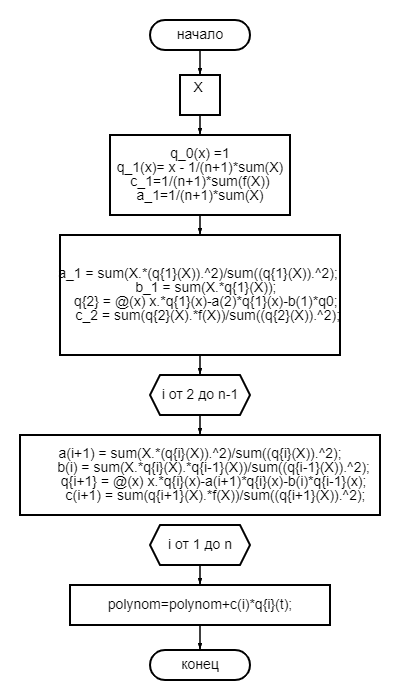
\includegraphics[scale=0.7]{diagram (6).png} 
 \end{center}
\caption{Блок-схема приближения полиномом Фурье} \label{Рис1}
\end{figure}


\newpage
\section{Численный анализ решения задачи}
\subsection{Исследование влияния гладкости на сходимость} 
По условию заданы функции $ y = x+sin(x)$ и $ y(x) = 3sign(x)x^{4}-8x^{3}-18x^{2}+6$, рассмотрим их на отрезке $[-1.3;1.05]$. Тогда для заданных функций строим полиномы Фурье с равномерной сеткой, таким образом, получаем график на рисунке \ref{Рис2}.
\begin{figure}[h!]
\begin{center}
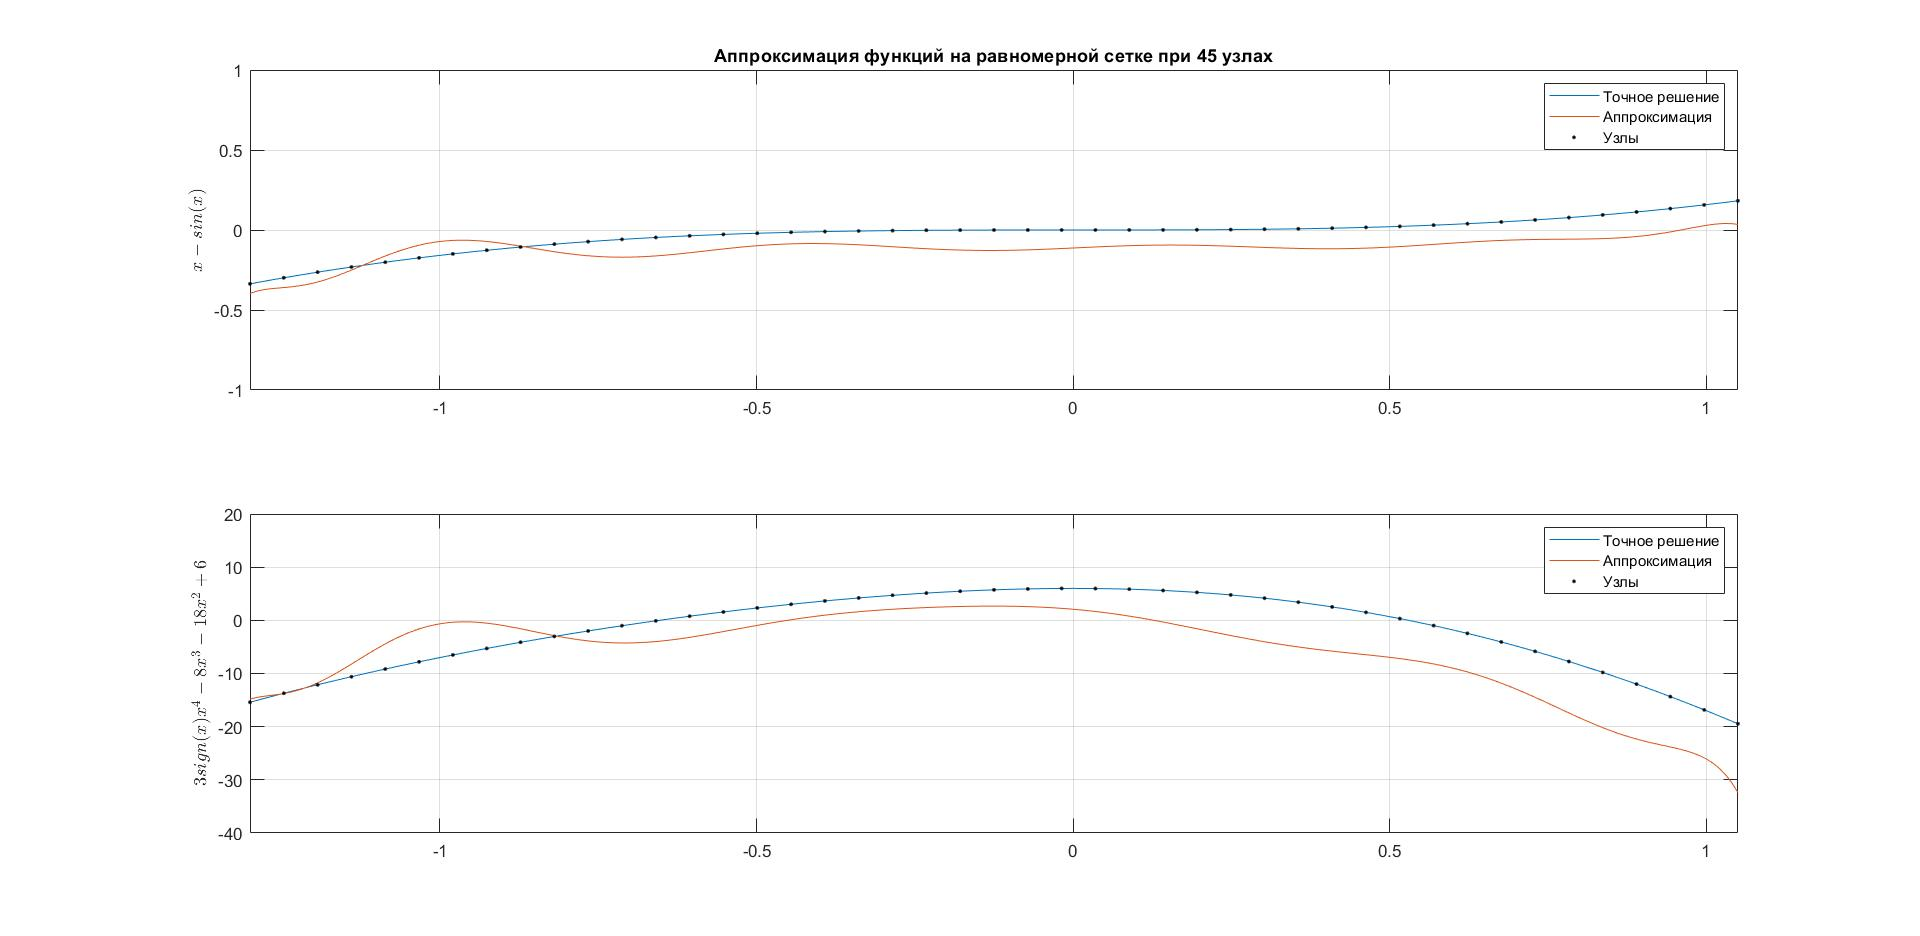
\includegraphics[scale=0.3]{функция и аппроксимация.jpg} 
\end{center}
\caption{График полиномов Фурье и исходных функций на заданном интервале} \label{Рис2}
\end{figure}\\
На данном этапе нельзя заметить, чтобы приближение какой-либо из функций было бы выполнено намного лучше.Однако видно, что аппроксимация гладкой функции ближе к ее настоящему графику.Чтобы более подробно рассмотреть влияние гладкости функции, рассмотрим график зависимости ошибки от координаты для двух функций при всё тех же условиях.
\begin{figure}[h!]
\begin{center}
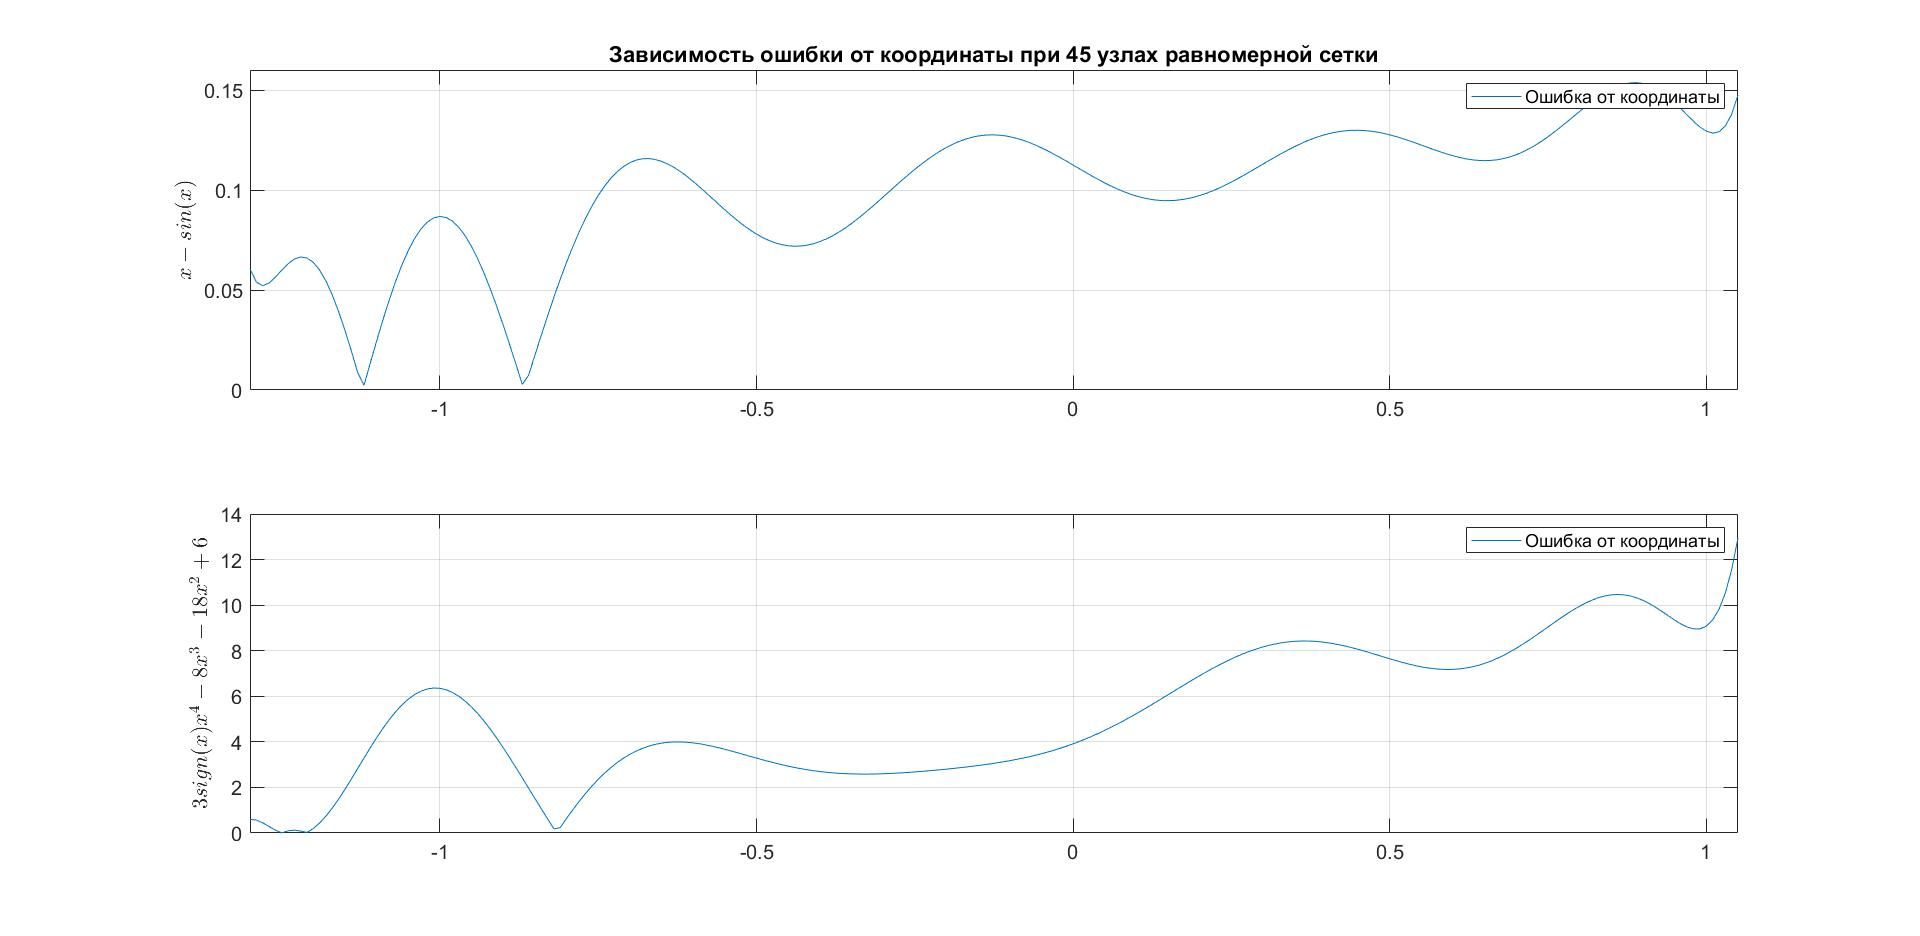
\includegraphics[scale=0.3]{зависимость ошибка от координаты.jpg} 
\end{center}
\caption{График зависимости ошибки от координаты} \label{Рис3}
\end{figure}\\
Можно увидеть на рисунке \ref{Рис3}, что ошибка для гладкой функции действительно является меньше.


\newpage

\section{Исследование влияния количества узлов на сходимость} 
\subsection{Чебышевская сетка}
\begin{figure}[h!]
\begin{center}
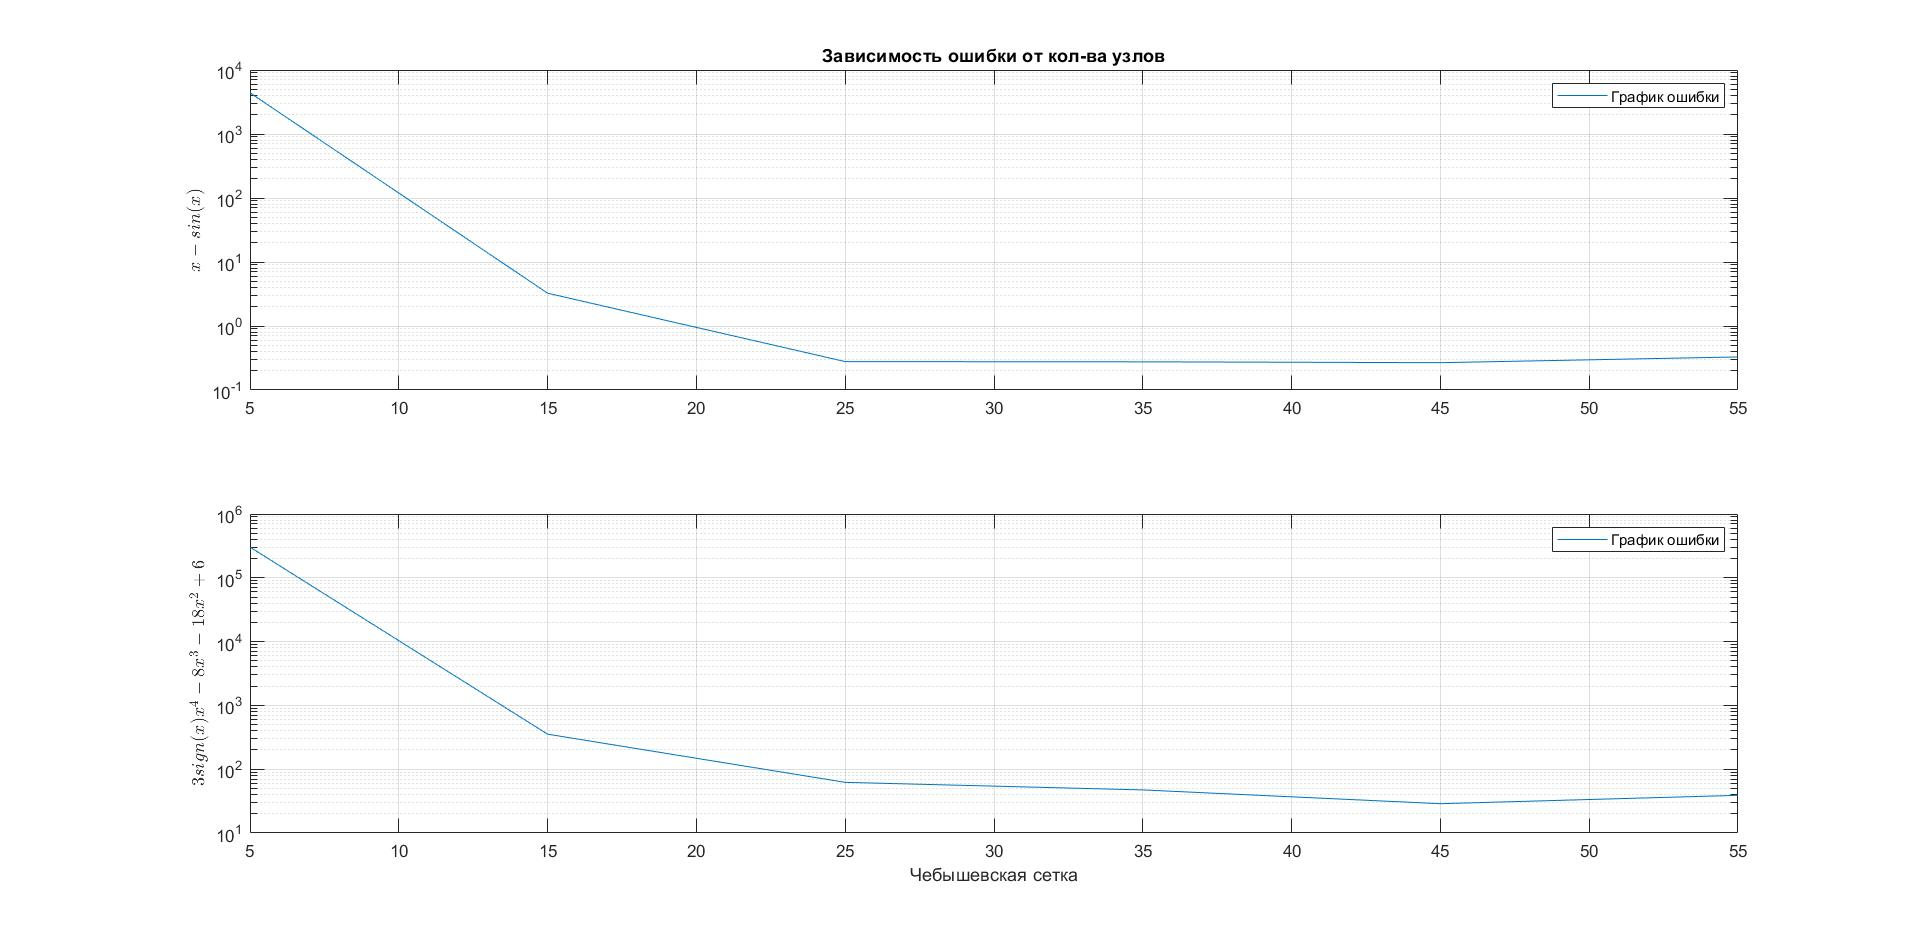
\includegraphics[scale=0.3]{зависимость ошибки от кол-ва узлов.jpg} 
\end{center}
\caption{Зависимость ошибки от кол-ва узлов для полиномов Фурье} \label{Рис4}
\end{figure}
 \begin{figure}[h!]
\begin{center}
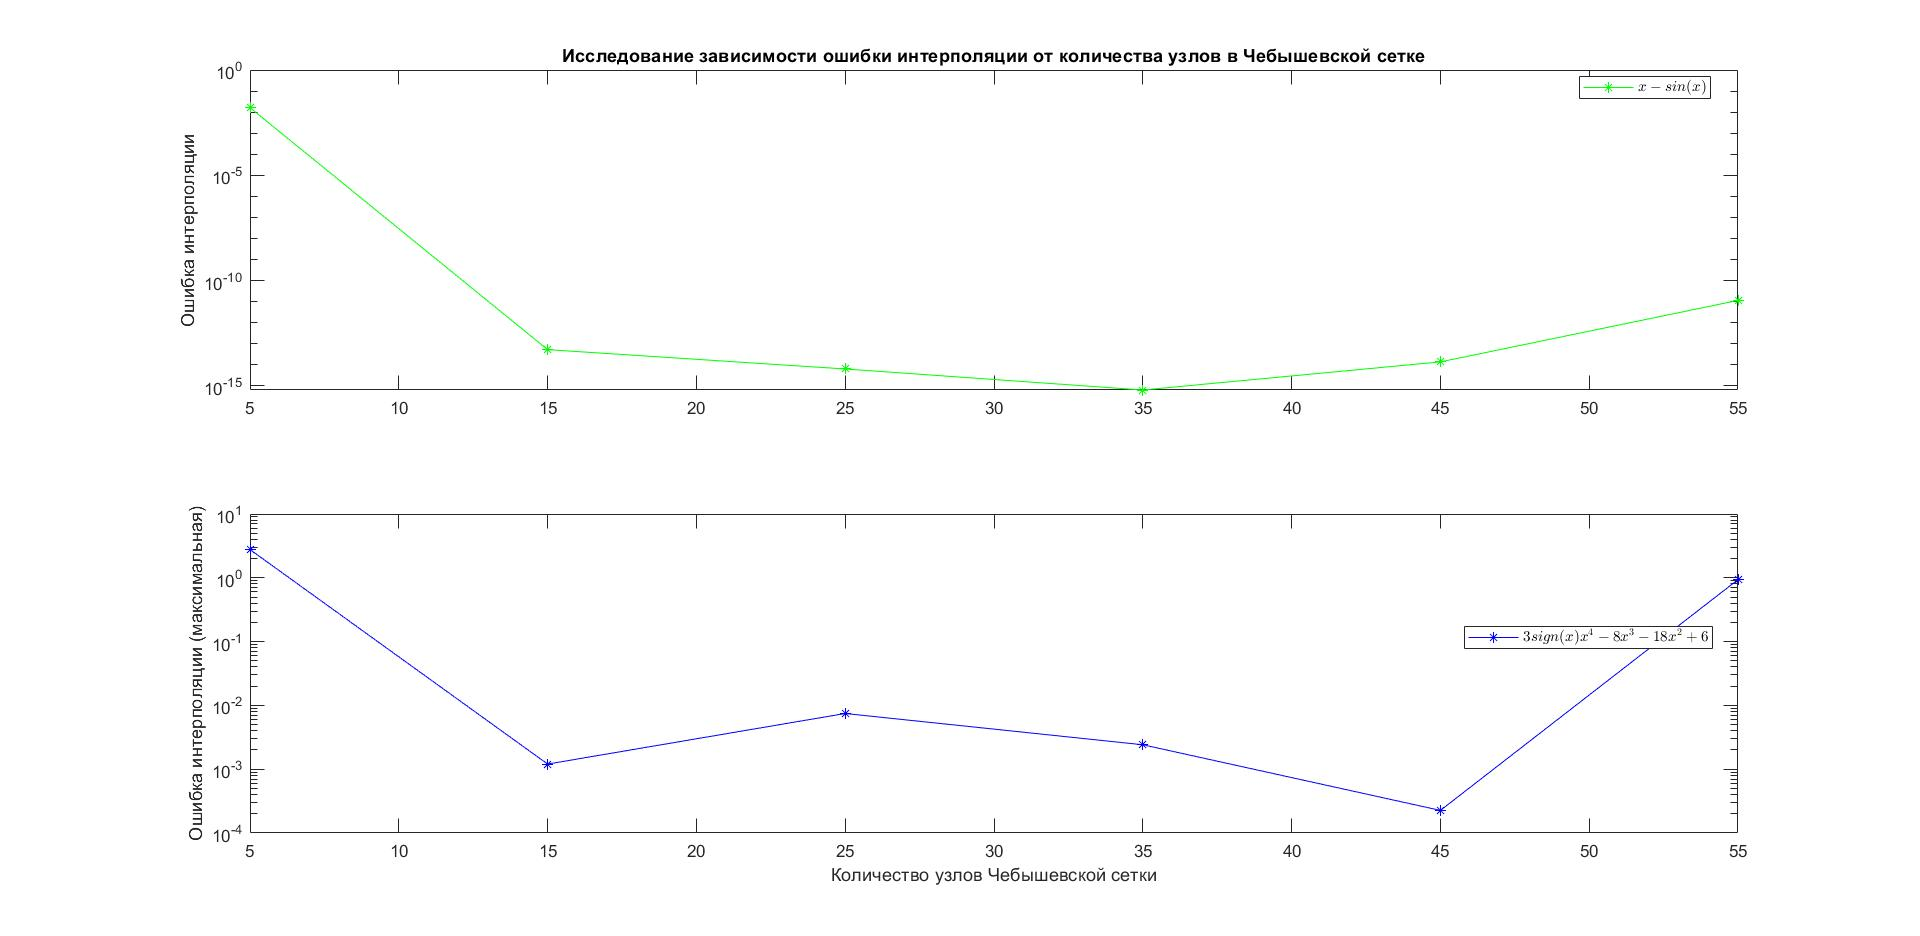
\includegraphics[scale=0.3]{кол-во узлов Чебышев.jpg} 
\end{center}
\caption{Зависимость ошибки от кол-ва узлов для полиномов Лагранжа} \label{Рис5}
\end{figure}
Теперь рассмотрим, как влияет количество узлов на величину погрешности и сделаем построения для Чебышевской сетки. На рисунке $\ref{Рис4}$ мы наблюдаем что для полиномов Фурье ошибка уменьшается при увеличении количества узлов сетки. Что для гладкой, что для функции с разрывом в производной тенденция одинакова.Однако, порядок ошибки больше у функции с разрывом производной. Сравним аппроксимацию полиномов Фурье с интерполяцией тех же функций полиномами Лагранжа. Как видим, на рисунке \ref{Рис5} зависимости очень похожи, но порядок приближения у полинома Лагранжа в разы лучше. Можно заметить, что для негладкой функций разбиением с самой "лучшей" ошибкой является разбиение 45, как в приближении Фурье, так и для Лагранжа. Также стоит отметить, что при преодолении определенной отметки количества разбиений погрешность полиномов Лагранжа начинает  сильно увеличиваться, чего не сказать о полиномах Фурье.


\subsection{Произвольная сетка}
\begin{figure}[h!]
\begin{center}
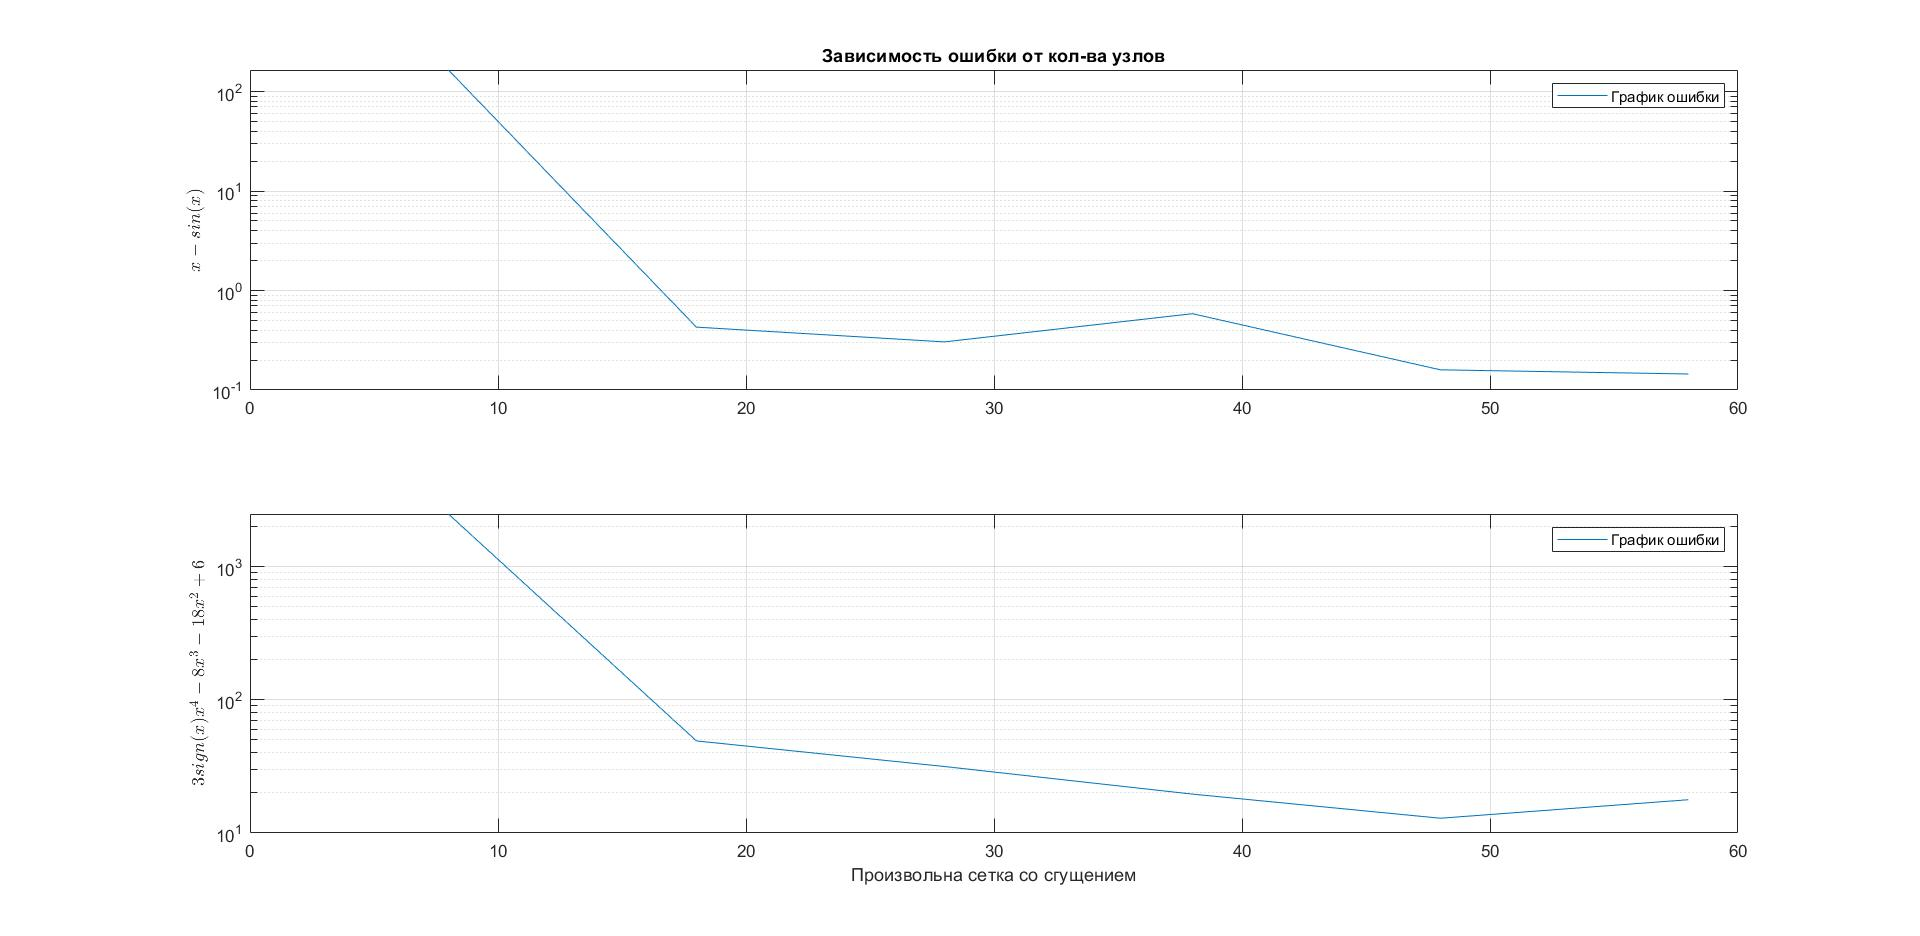
\includegraphics[scale=0.3]{ависимость ошибки от кол-ва узлов произвольная сетка.jpg}  
\end{center}
\caption{Зависимость ошибки от кол-ва узлов для полиномов Фурье} \label{Рис6}
\end{figure}
 \begin{figure}[h!]
\begin{center}
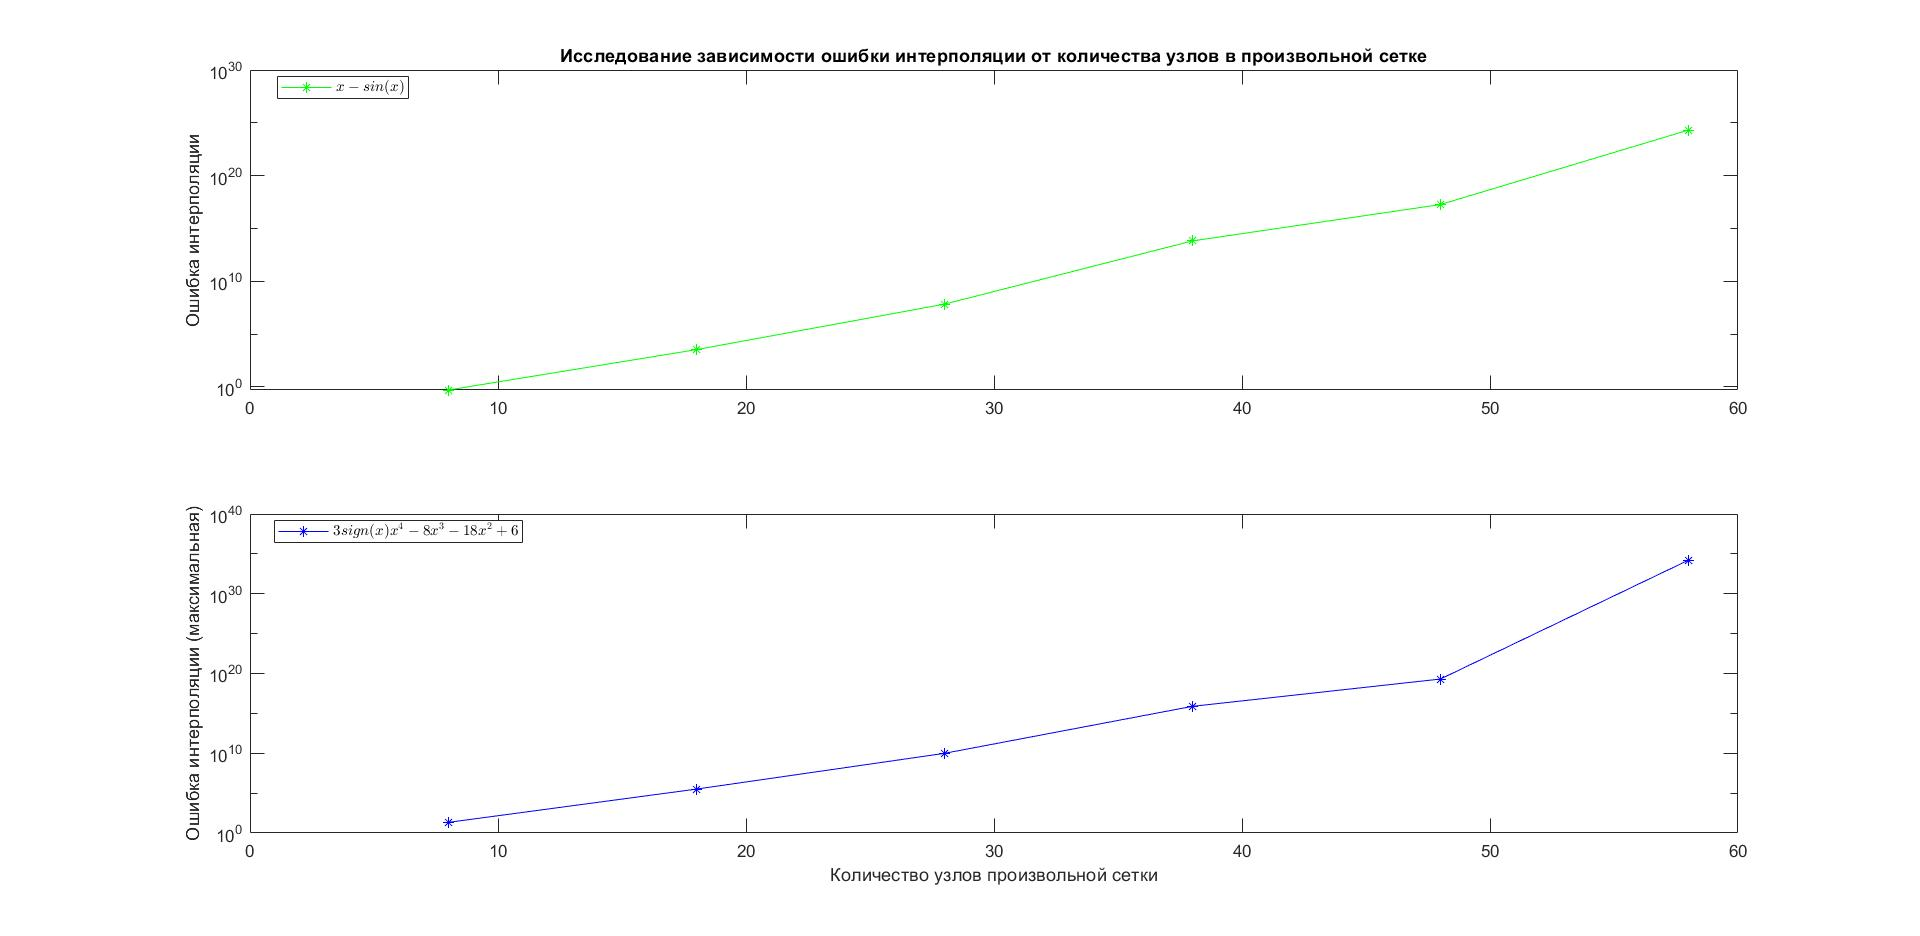
\includegraphics[scale=0.3]{кол-во узлов Произвольная.jpg} 
\end{center}
\caption{Зависимость ошибки от кол-ва узлов для полиномов Лагранжа} \label{Рис7}
\end{figure}

Рассмотрим теперь графики зависимоси ошибки от количества узлов на произвольной сетке. Как можно заметить на рисунке \ref{Рис6}, общая характеристика графиков примерно похожа на выше рассмотренные случаи (рисунок \ref{Рис4}): ошибка уменьшается, порядок ошибки у гладкой функции меньше. Однако, в сравнении с интерполяцией Лагранжа (рисунок \ref{Рис7}) видна большая разница. При увеличении количества узлов приближение полиномом Лагранжа "ухудшается".


\newpage
\section{Краткие выводы} 

\begin{itemize}
  \item Аппроксимация полиномами Фурье дает неплохой результат, если взять достаточное количество узлов.
  \item Полином Лагранжа во многом превосходит приближение полиномами Фурье для данных функций, однако стоит отметить, что при большом количестве узлов полиномы Фурье могут дать лУчшее приближение.
  \item При сравнении гладкой функции и функции с разрывом в производной было понято, что аппроксимацию лучше проводить для гладкой функции, т.к. она даст лучший результат с меньшим значением ошибки.
  
\end{itemize}


\end{document} % КОНЕЦ ДОКУМЕНТА !

